\documentclass{beamer}
\usepackage{tikz,amsmath,hyperref,graphicx,stackrel,animate,tipa}
\usetikzlibrary{positioning,shadows,arrows,shapes,calc}
\newcommand{\ipa}[1]{\textipa{#1}}
\newcommand{\argmax}{\operatornamewithlimits{argmax}}
\newcommand{\argmin}{\operatornamewithlimits{argmin}}
\mode<presentation>{\usetheme{Frankfurt}}
\DeclareMathOperator*{\softmax}{softmax}
\AtBeginSection[]
{
  \begin{frame}<beamer>
    \frametitle{Outline}
    \tableofcontents[currentsection,currentsubsection]
  \end{frame}
}
\title{Lecture 16: Numerical Issues in Training HMMs}
\author{Mark Hasegawa-Johnson\\All content~\href{https://creativecommons.org/licenses/by/4.0/}{CC-BY 4.0} unless otherwise specified.}
\date{ECE 417: Multimedia Signal Processing, Fall 2021}  
\begin{document}

% Title
\begin{frame}
  \maketitle
\end{frame}

% Title
\begin{frame}
  \tableofcontents
\end{frame}

%%%%%%%%%%%%%%%%%%%%%%%%%%%%%%%%%%%%%%%%%%%%
\section[Review]{Review: Hidden Markov Models}
\setcounter{subsection}{1}

\begin{frame}
  \frametitle{The Three Problems for an HMM}
  \begin{center}
    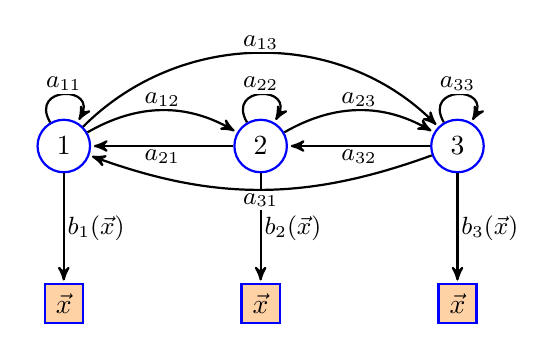
\begin{tikzpicture}[->,>=stealth',shorten >=1pt,auto,node distance=3cm,thick,
        state/.style={circle,thick,draw=blue,text=black,text centered,text width=0.25cm},
        obs/.style={rectangle,thick,draw=blue,text=black,fill=orange!35!white,text centered,text width=0.25cm}
      ]
      \node[state] (q1) at (0,0) {1};
      \node[state] (q2) at (2.5,0) {2};
      \node[state] (q3) at (5,0) {3};
      \node[obs] (x1) at (0,-2) {$\vec{x}$};
      \node[obs] (x2) at (2.5,-2) {$\vec{x}$};
      \node[obs] (x3) at (5,-2) {$\vec{x}$};
      \path[every node/.style={font=\sffamily\small,
  	  fill=white,inner sep=1pt}]
      (q1) edge [out=120,in=60,looseness=4] node {$a_{11}$} (q1)
      edge [out=30,in=150] node {$a_{12}$} (q2)
      edge [out=45,in=135] node {$a_{13}$} (q3)
      edge [out=-90,in=90] node {$b_1(\vec{x})$} (x1)
      (q2) edge [out=120,in=60,looseness=4] node {$a_{22}$} (q2)
      edge [out=180,in=0] node {$a_{21}$} (q1)
      edge [out=30,in=150] node {$a_{23}$} (q3)
      edge [out=-90,in=90] node {$b_2(\vec{x})$} (x2)
      (q3) edge [out=120,in=60,looseness=4] node {$a_{33}$} (q3)
      edge [out=180,in=0] node {$a_{32}$} (q2)
      edge [out=-160,in=-20] node {$a_{31}$} (q1)
      edge [out=-90,in=90] node {$b_3(\vec{x})$} (x3);
    \end{tikzpicture}
  \end{center}
  \begin{enumerate}
  \item {\bf Recognition:} Given two different HMMs, $\Lambda_1$ and
    $\Lambda_2$, and an observation sequence $X$.  Which HMM was more
    likely to have produced $X$?  In other words, 
    $p(X|\Lambda_1)>p(X|\Lambda_2)$?
  \item {\bf Segmentation:} What is $p(Q|X,\Lambda)$?
  \item {\bf Training:} Given an initial HMM $\Lambda$, and an
    observation sequence $X$, can we find $\Lambda'$ such that
    $p(X|\Lambda') > p(X|\Lambda)$?
  \end{enumerate}
\end{frame}

\begin{frame}
  \frametitle{Recognition: The Forward Algorithm}

  Definition: $\alpha_t(i) \equiv p(\vec{x}_1,\ldots,\vec{x}_t,q_t=i|\Lambda)$.  Computation:
  \begin{enumerate}
  \item {\bf Initialize:}
    \[
    \alpha_1(i) = \pi_i b_i(\vec{x}_1),~~~1\le i\le N
    \]
  \item {\bf Iterate:}
    \begin{align*}
      \alpha_{t}(j) &= \sum_{i=1}^N \alpha_{t-1}(i) a_{ij}b_j(\vec{x}_t),~~1\le j\le N,~2\le t\le T
    \end{align*}
  \item {\bf Terminate:}
    \[
    p(X|\Lambda) = \sum_{i=1}^N \alpha_T(i)
    \]
  \end{enumerate}
\end{frame}
  
\begin{frame}
  \frametitle{Segmentation: The Backward Algorithm}

  Definition: $\beta_t(i) \equiv p(\vec{x}_{t+1},\ldots,\vec{x}_T|q_t=i,\Lambda)$.  Computation:
  \begin{enumerate}
  \item {\bf Initialize:}
    \[
    \beta_T(i) = 1,~~~1\le i\le N
    \]
  \item {\bf Iterate:}
    \begin{align*}
      \beta_{t}(i) &= \sum_{j=1}^N a_{ij}b_j(\vec{x}_{t+1})\beta_{t+1}(j),~~1\le i\le N,~1\le t\le T-1
    \end{align*}
  \item {\bf Terminate:}
    \[
    p(X|\Lambda) = \sum_{i=1}^N \pi_ib_i(\vec{x}_1)\beta_1(i)
    \]
  \end{enumerate}
\end{frame}

\begin{frame}
  \frametitle{Segmentation: State and Segment Posteriors}

  \begin{enumerate}
  \item {\bf The State Posterior:}
    \begin{align*}
      \gamma_t(i) & = p(q_t=i|X,\Lambda)
      = \frac{\alpha_t(i)\beta_t(i)}{\sum_{k=1}^N\alpha_t(k)\beta_t(k)}
    \end{align*}
  \item {\bf The Segment Posterior:}
    \begin{align*}
      \xi_t(i,j) & = p(q_t=i,q_{t+1}=j|X,\Lambda)\\
      &= \frac{\alpha_t(i)a_{ij}b_j(\vec{x}_{t+1})\beta_{t+1}(j)}{\sum_{k=1}^N\sum_{\ell=1}^N\alpha_t(k)a_{k\ell}b_\ell(\vec{x}_{t+1})\beta_{t+1}(\ell)}
    \end{align*}
  \end{enumerate}
\end{frame}

\begin{frame}
  \frametitle{Training: The Baum-Welch Algorithm}

  \begin{enumerate}
  \item {\bf Transition Probabilities:}
    \begin{align*}
      a_{ij}' &=\frac{\sum_{t=1}^{T-1} \xi_t(i,j)}{\sum_{j=1}^N\sum_{t=1}^{T-1}\xi_t(i,j)}
    \end{align*}
  \item {\bf Gaussian Observation PDFs:}
    \begin{displaymath}
      \vec\mu_{i}' = \frac{\sum_{t=1}^T\gamma_t(i)\vec{x}_{t}}{\sum_{t=1}^T\gamma_t(i)}
    \end{displaymath}
    \begin{displaymath}
      \Sigma_{i}' = \frac{\sum_{t=1}^T\gamma_t(i)(\vec{x}_{t}-\vec\mu_{i})(\vec{x}_t-\vec\mu_i)^T}{\sum_{t=1}^T\gamma_t(i)}
    \end{displaymath}
  \end{enumerate}
\end{frame}

%%%%%%%%%%%%%%%%%%%%%%%%%%%%%%%%%%%%%%%%%%%%
\section[Issues]{Numerical Issues in the Training of an HMM}
\setcounter{subsection}{1}

\begin{frame}
  \frametitle{Numerical Issues in the  Training  of an HMM}
  \begin{itemize}
  \item {\bf Flooring the observation pdf}: $e^{-\frac{1}{2}(\vec{x}-\vec\mu)^T\Sigma^{-1}(\vec{x}-\vec\mu)}$ can be very small.
  \item {\bf Scaled forward-backward algorithm:} $a_{ij}^T$ can be very small.
  \item {\bf Zero denominators:} Sometimes $\sum_i\alpha_t(i)\beta_t(i)$ is zero.
  \item {\bf Tikhonov regularization:} Re-estimation formulae can result in $|\Sigma_i|=0$.
  \end{itemize}
\end{frame}

%%%%%%%%%%%%%%%%%%%%%%%%%%%%%%%%%%%%%%%%%%%%
\section[Observations]{Flooring the observation pdf}
\setcounter{subsection}{1}

\begin{frame}
  \frametitle{Flooring the observation pdf: Why is it necessary?}

  Suppose that $b_j(\vec{x})$ is Gaussian:
  \begin{displaymath}
    b_j(\vec{x})=
    \frac{1}{\prod_{d=1}^D\sqrt{2\pi\sigma_{jd}^2}}e^{-\frac{1}{2}\sum_{d=1}^D\frac{(x_d-\mu_{jd})^2}{\sigma_{jd}^2}}
  \end{displaymath}
  Suppose that $D\approx 30$.  Then:
  \centerline{\begin{tabular}{|l|c|c|}\hline
      Average distance from the mean & Observation pdf \\
      $\frac{x_d-\mu_{jd}}{\sigma_{jd}}$ &
      $\frac{1}{(2\pi)^{15}}e^{-\frac{1}{2}\prod_{d=1}^D\left(\frac{x_d-\mu_{jd}}{\sigma_{jd}}\right)^2}$ \\\hline 
      1 & $\frac{1}{(2\pi)^{15}}e^{-15}\approx 10^{-19}$\\
      3 & $\frac{1}{(2\pi)^{15}}e^{-135}\approx 10^{-71}$\\
      5 & $\frac{1}{(2\pi)^{15}}e^{-375}\approx 10^{-175}$\\
      7 & $\frac{1}{(2\pi)^{15}}e^{-735}\approx 10^{-331}$\\\hline
  \end{tabular}}
\end{frame}

\begin{frame}
  \frametitle{Why is that a problem?}

  \begin{itemize}
  \item IEEE single-precision floating  point: smallest number is $10^{-38}$.
  \item IEEE double-precision floating point (numpy): smallest number is $10^{-324}$.
  \end{itemize}
\end{frame}

\begin{frame}
  \frametitle{Why is that a problem?}

  \begin{align*}
    \alpha_{t}(j) &= \sum_{i=1}^N \alpha_{t-1}(i) a_{ij}b_j(\vec{x}_t),~~1\le j\le N,~2\le t\le T
  \end{align*}
  \begin{itemize}
  \item If some (but not all) $a_{ij}=0$, and some (but not all)
    $b_j(\vec{x})=0$, then it's possible that all $a_{ij}b_j(\vec{x})=0$.
  \item In that case, it's possible to get $\alpha_t(j)=0$ for all $j$.
  \item In that case, recognition crashes.
  \end{itemize}
\end{frame}

\begin{frame}
  \frametitle{One possible solution: Floor the observation pdf}

  There are many possible solutions, including scaling solutions
  similar to the scaled forward that I'm about to introduce.  But for
  the MP, I recommend a simple solution: floor the observation pdf.  Thus:

  \begin{displaymath}
    b_j(\vec{x}) = \max\left(\mbox{floor}, {\mathcal N}(\vec{x}|\vec\mu_j,\Sigma_j)\right)
  \end{displaymath}

  The floor needs to be much larger than $10^{-324}$, but much smaller
  than ``good'' values of the Gaussian (values observed for
  non-outlier spectra).  In  practice, a good choice seems to be
  \[
  \mbox{floor}=10^{-100}
  \]
\end{frame}

\begin{frame}
  \frametitle{Result example}

  Here is $\ln b_i(\vec{x}_t)$, plotted as a function of $i$ and $t$,
  for the words ``one,'' ``two,'' and ``three.''
  \centerline{\includegraphics[height=2.5in]{log_b.png}}
\end{frame}

%%%%%%%%%%%%%%%%%%%%%%%%%%%%%%%%%%%%%%%%%%%%
\section[Scaling]{Scaled Forward-Backward Algorithm}
\setcounter{subsection}{1}

\begin{frame}
  \frametitle{The Forward Algorithm}

  Definition: $\alpha_t(i) \equiv p(\vec{x}_1,\ldots,\vec{x}_t,q_t=i|\Lambda)$.  Computation:
  \begin{enumerate}
  \item {\bf Initialize:}
    \[
    \alpha_1(i) = \pi_i b_i(\vec{x}_1),~~~1\le i\le N
    \]
  \item {\bf Iterate:}
    \begin{align*}
      \alpha_{t}(j) &= \sum_{i=1}^N \alpha_{t-1}(i) a_{ij}b_j(\vec{x}_t),~~1\le j\le N,~2\le t\le T
    \end{align*}
  \item {\bf Terminate:}
    \[
    p(X|\Lambda) = \sum_{i=1}^N \alpha_T(i)
    \]
  \end{enumerate}
\end{frame}


\begin{frame}
  \frametitle{Numerical Issues}

  The forward algorithm is susceptible to massive floating-point
  underflow problems. Consider this equation:
  \begin{align*}
    \alpha_{t}(j) &= \sum_{i=1}^N \alpha_{t-1}(i) a_{ij}b_j(\vec{x}_t)\\
    &= \sum_{q_1=1}^N\cdots\sum_{q_{t-1}=1}^N \pi_{q_1}b_{q_1}(\vec{x}_1)\cdots
    a_{q_{t-1}q_{t}}b_{q_t}(\vec{x}_t)
  \end{align*}
  First, suppose that $b_q(x)$ is discrete, with
  $k\in\left\{1,\ldots,K\right\}$.  Suppose $K\approx 1000$ and
  $T\approx 100$, in that case, each $\alpha_t(j)$ is:
  \begin{itemize}
  \item The sum of $N^T$ different terms, each of which is
  \item the product of $T$ factors, each of which is
  \item the product of two probabilities: $a_{ij}\sim\frac{1}{N}$ times
    $b_j(x)\sim\frac{1}{K}$, so
    \begin{displaymath}
      \alpha_T(j) \approx N^T\left(\frac{1}{NK}\right)^{T} \approx \frac{1}{K^T}\approx 10^{-300}
    \end{displaymath}
  \end{itemize}
\end{frame}

\begin{frame}
  \frametitle{The Solution: Scaling}

  The solution is to just re-scale $\alpha_t(j)$ at each time step, so
  it never gets really small:
  \begin{align*}
    \hat\alpha_{t}(j) &=
    \frac{\sum_{i=1}^N \hat\alpha_{t-1}(i) a_{ij}b_j(\vec{x}_t)}
         {\sum_{\ell=1}^N\sum_{i=1}^N \hat\alpha_{t-1}(i) a_{i\ell}b_\ell(\vec{x}_t)}
  \end{align*}

  Now the problem is\ldots if $\alpha_t(j)$ has been re-scaled, how do
  we perform recognition?  Remember we used to have
  $p(X|\Lambda)=\sum_i\alpha_t(i)$.  How can we get $p(X|\Lambda)$
  now?
\end{frame}

\begin{frame}
  \frametitle{What exactly is alpha-hat?}

  Let's look at this in more detail.  $\alpha_t(j)$ is defined to be
  $p(\vec{x}_1,\ldots,\vec{x}_t,q_t=j|\Lambda)$.  Let's define a
  ``scaling term,'' $g_t$, equal to the denominator in the scaled
  forward algorithm.  So, for example, at time $t=1$ we have:
  \begin{displaymath}
  g_1 = \sum_{\ell=1}^N \alpha_1(\ell)= \sum_{\ell=1}^N p(\vec{x}_1,q_1=\ell|\Lambda)
  = p(\vec{x}_1|\Lambda)
  \end{displaymath}
  and therefore
  \begin{displaymath}
  \hat\alpha_1(i) = \frac{\alpha_1(i)}{g_1} 
  = \frac{p(\vec{x}_1,q_1=i|\Lambda)}{p(\vec{x}_1|\Lambda)}
  = p(q_1=i|\vec{x}_1,\Lambda)
  \end{displaymath}
\end{frame}

\begin{frame}
  \frametitle{What exactly is alpha-hat?}
  At time $t$, we need a new intermediate variable.  Let's call it $\tilde\alpha_t(j)$:
  \begin{align*}
  \tilde\alpha_t(j) &= \sum_{i=1}^N \hat\alpha_{t-1}(i) a_{ij}b_j(\vec{x}_t)\\
  &= \sum_{i=1}^N p(q_{t-1}=i|\vec{x}_1,\ldots,\vec{x}_{t-1},\Lambda)p(q_t=j|q_{t-1}=i)p(\vec{x}_t|q_t=j)\\
  &= p(q_{t}=j,\vec{x}_t|\vec{x}_1,\ldots,\vec{x}_{t-1},\Lambda)\\
  g_t &= \sum_{\ell=1}^N \tilde\alpha_t(\ell) = p(\vec{x}_t|\vec{x}_1,\ldots,\vec{x}_{t-1},\Lambda)
  \end{align*}
  \begin{displaymath}
  \hat\alpha_t(j) = \frac{\tilde\alpha_t(j)}{g_t}
  = \frac{p(\vec{x}_t,q_t=j|\vec{x}_1,\ldots,\vec{x}_{t-1},\Lambda)}{p(\vec{x}_t|\vec{x}_1,\ldots,\vec{x}_{t-1},\Lambda)}
  = p(q_t=j|\vec{x}_1,\ldots,\vec{x}_t,\Lambda)
  \end{displaymath}
\end{frame}

\begin{frame}
  \frametitle{Scaled Forward Algorithm: The Variables}

  So we have not just one, but three new variables:
  \begin{enumerate}
  \item The intermediate forward probability:
    \begin{displaymath}
      \tilde\alpha_t(j) = p(q_t=j,\vec{x}_t|\vec{x}_1,\ldots,\vec{x}_{t-1},\Lambda)
    \end{displaymath}
  \item The scaling factor:
    \begin{displaymath}
      g_t = p(\vec{x}_t|\vec{x}_1,\ldots,\vec{x}_{t-1},\Lambda)
    \end{displaymath}
  \item The scaled forward probability:
    \begin{displaymath}
      \hat\alpha_t(j) = p(q_t=j|\vec{x}_1,\ldots,\vec{x}_{t},\Lambda)
    \end{displaymath}
  \end{enumerate}
\end{frame}

\begin{frame}
  \frametitle{The Solution}

  The second of those variables is interesting because we want $p(X|\Lambda)$, which
  we can now get from the $g_t$s---we no longer actually need the $\alpha$s for this!
  \begin{displaymath}
    p(X|\Lambda) = p(\vec{x}_1|\Lambda )p(\vec{x}_2|\vec{x}_1,\Lambda)p(\vec{x}_3|\vec{x}_1,\vec{x}_2,\Lambda )\cdots= \prod_{t=1}^T g_t
  \end{displaymath}
  But that's still not useful, because if each $g_t\sim 10^{-19}$,
  then multiplying them all together will result in floating point
  underflow.  So instead, it is better to compute
  \begin{align*}
    \ln p(X|\Lambda) = \sum_{t=1}^T \ln g_t
  \end{align*}
\end{frame}

\begin{frame}
  \frametitle{The Scaled Forward Algorithm}

  \begin{enumerate}
  \item {\bf Initialize:}
    \[
    \hat\alpha_1(i) = \frac{1}{g_1}\pi_i b_i(\vec{x}_1)
    \]
  \item {\bf Iterate:}
    \begin{align*}
      \tilde\alpha_{t}(j) &= \sum_{i=1}^N \hat\alpha_{t-1}(i) a_{ij}b_j(\vec{x}_t)\\
      g_t &= \sum_{j=1}^N \tilde\alpha_t(j)\\
      \hat\alpha_{t}(j) &= \frac{1}{g_t}\tilde\alpha_t(j)
    \end{align*}
  \item {\bf Terminate:}
    \[
    \ln p(X|\Lambda) = \sum_{t=1}^T \ln g_t
    \]
  \end{enumerate}
\end{frame}

\begin{frame}
  \frametitle{Result example}

  Here are $\hat\alpha_t(i)$ and $\ln g_t$, plotted as a function of $i$ and $t$, for
  the words ``one,'' ``two,'' and ``three.''
  \centerline{\includegraphics[height=2.5in]{alphahat.png}}
\end{frame}

%%%%%%%%%%%%%%%%%%%%%%%%%%%%%%%%%%%%%%%%%%%%
%\section[Segmentation]{Segmentation: The Viterbi Algorithm}
%\setcounter{subsection}{1}
%
%\begin{frame}
%  \frametitle{What About State Sequences?}
%
%  \begin{itemize}
%  \item Remember when we first derived $\gamma_t(i)$, I pointed out a
%    problem: $\gamma_t(i)$ only tells us about one frame at a time!
%    It doesn't tell us anything about the probability of a sequence of
%    states, covering a sequence of frames.
%  \item Today, let's find a complete solution.  Let's find the most
%    likely state sequence covering the entire utterance:
%    \[
%    Q^*  = \argmax_Q p(Q,X|\Lambda)
%    \]
%  \end{itemize}
%\end{frame}
%
%\begin{frame}
%  \frametitle{The Max-Probability State Sequence}
%
%  The problem of finding the max-probability state sequence is just as
%  hard as the problem of finding $p(X|\Lambda)$, for exactly the same
%  reason:
%  \begin{align*}
%    \max_Q p(Q,X|\Lambda) &= \max_{q_T=1}^N\cdots\max_{q_1=1}^N p(Q,X|\Lambda)
%  \end{align*}
%  which has complexity ${\mathcal O}\left\{N^T\right\}$.
%\end{frame}
%\begin{frame}
%  \frametitle{The Viterbi Algorithm}
%  
%  Remember that we solved the recognition probability using a
%  divide-and-conquer kind of dynamic programming algorithm, with the
%  intermediate variable
%  \begin{align*}
%  \alpha_t(j) &\equiv p(\vec{x}_1,\ldots,\vec{x}_t,q_t=j|\Lambda)\\
%  &=\sum_{q_{t-1}}\cdots\sum_{q_1}
%  p(\vec{x}_1,\ldots,\vec{x}_t,q_1,\ldots,q_{t-1},q_t=j|\Lambda)
%  \end{align*}
%  The segmentation problem is solved using a similar dynamic
%  programming algorithm called the Viterbi algorithm, with a slightly
%  different intermediate variable:
%  \[
%  \delta_t(j)\equiv \max_{q_{t-1}}\cdots\max_{q_1}
%  p(\vec{x}_1,\ldots,\vec{x}_t,q_1,\ldots,q_{t-1},q_t=j|\Lambda)
%  \]
%\end{frame}
%
%\begin{frame}
%  \frametitle{The Viterbi Algorithm}
%  Keeping in mind the definition
%  $\delta_t(j)\equiv\max_{q_{t-1}}\cdots\max_{q_1}p(\vec{x}_1,\ldots,\vec{x}_t,q_1,\ldots,q_{t-1},q_t=j|\Lambda)$,
%  we can devise an efficient algorithm to compute it:
%  \begin{enumerate}
%  \item {\bf Initialize:}
%    \[
%    \delta_1(i) = \pi_i b_i(\vec{x}_1)
%    \]
%  \item {\bf Iterate:}
%    \begin{align*}
%      \delta_{t}(j) &= \max_{i=1}^N \delta_{t-1}(i) a_{ij}b_j(\vec{x}_t)
%    \end{align*}
%  \item {\bf Terminate:}
%    The maximum-probability final state is $q_T^* = \argmax_{j=1}^N \delta_T(j)$.  But what
%    are the best states at all of the previous time steps?
%  \end{enumerate}
%\end{frame}
%
%\begin{frame}
%  \frametitle{Backtracing}
%
%  We can find the optimum states at all times, $q_t^*$, by keeping a
%  {\bf backpointer} $\psi_t(j)$ from every time step.  The backpointer
%  points to the state at time $t-1$ that is most likely to have
%  preceded state $j$ at time $t$:
%  \begin{align*}
%    \psi_{t}(j) &= \argmax_i\cdots\max_{q_1}p(\vec{x}_1,\ldots,\vec{x}_t,q_1,\ldots,q_{t-1}=i,q_t=j|\Lambda)\\
%   &= \argmax_{i=1}^N \delta_{t-1}(i) a_{ij}b_j(\vec{x}_t)
%  \end{align*}
%\end{frame}

%\begin{frame}
%  \frametitle{Backtracing}
%
%  If we have the backpointers available, then we can get the entire
%  maximum-probability state sequence by {\bf backtracing} after we
%  terminate:
%  \begin{itemize}
%  \item {\bf Terminate:} Once we get to time $t=T$, we choose the most
%    probable final state.
%    \begin{itemize}
%    \item If we already know which state we want to end in, then we
%      just choose that state as $q_T^*$.
%    \item If we don't already know, then we choose
%      $q_T^*=\argmax_{j}\delta_T(j)$
%    \end{itemize}
%  \item {\bf Backtrace:} Having found the final state, we work
%    backward, by way of the {\bf backpointers}, $\psi_t(j)$:
%    \begin{align*}
%      q_t^* &= \psi_{t+1}\left(q_{t+1}^*\right),~~~T-1\ge t\ge 1
%    \end{align*}
%  \end{itemize}
%\end{frame}
%
%\begin{frame}
%  \frametitle{The Viterbi Algorithm}
%  \begin{enumerate}
%  \item {\bf Initialize:}
%    \[
%    \delta_1(i) = \pi_i b_i(\vec{x}_1)
%    \]
%  \item {\bf Iterate:}
%    \begin{align*}
%      \delta_{t}(j) &= \max_{i=1}^N \delta_{t-1}(i) a_{ij}b_j(\vec{x}_t)\\
%      \psi_{t}(j) &= \argmax_{i=1}^N \delta_{t-1}(i) a_{ij}b_j(\vec{x}_t)
%    \end{align*}
%  \item {\bf Terminate:}
%    \begin{align*}
%      q_T^* &= \argmax_{j=1}^N \delta_T(j)
%    \end{align*}
%  \item {\bf Backtrace:}
%    \begin{align*}
%      q_t^* &= \psi_{t+1}\left(q_{t+1}^*\right)
%    \end{align*}
%  \end{enumerate}
%\end{frame}
%
%\begin{frame}
%  \frametitle{Example}
%  \centerline{\includegraphics[height=2.5in]{exp/An_example_of_HMM.png}}
%  \begin{tiny}
%    An example of HMM, GFDL by Reelsun, 2012,
%    \url{https://commons.wikimedia.org/wiki/File:An_example_of_HMM.png}
%  \end{tiny}
%\end{frame}
%
%\begin{frame}
%  \frametitle{Example}
%  \centerline{\animategraphics[loop,controls,width=4.5in]{1}{exp/Viterbi_animated_demo-}{0}{4}}
%  \begin{tiny}
%    Viterbi animated demo, GFDL by Reelsun, 2012,
%    \url{https://commons.wikimedia.org/wiki/File:Viterbi_animated_demo.gif}
%  \end{tiny}
%\end{frame}
%
%\begin{frame}
%  \frametitle{Numerical Problems}
%
%  Viterbi algorithm has the same floating-point underflow problems as
%  the Forward algorithm.  But this time, there is an easy solution,
%  because the log of the max is equal to the max of the log:
%  \begin{align*}
%    \ln\delta_{t}(j) &= \ln\left(\max_{i=1}^N \delta_{t-1}(i) a_{ij}b_j(\vec{x}_t)\right)\\
%    &= \max_{i=1}^N\left(\ln\delta_{t-1}(i)+ \ln a_{ij}+ \ln b_j(\vec{x}_t)\right)
%  \end{align*}
%\end{frame}
%      
%\begin{frame}
%  \frametitle{The Log-Viterbi Algorithm}
%
%  \begin{enumerate}
%  \item {\bf Initialize:}
%    \[
%    \ln\delta_1(i) = \ln\pi_i +\ln b_i(\vec{x}_1)
%    \]
%  \item {\bf Iterate:}
%    \begin{align*}
%      \ln\delta_{t}(j) &= \max_{i=1}^N \left(\ln\delta_{t-1}(i) +\ln a_{ij}+ \ln b_j(\vec{x}_t)\right)\\
%      \psi_{t}(j) &= \argmax_{i=1}^N \left(\ln\delta_{t-1}(i) +\ln a_{ij}+ \ln b_j(\vec{x}_t)\right)
%    \end{align*}
%  \item {\bf Terminate:}
%    Choose the known final state $q_T^*$.
%  \item {\bf Backtrace:}
%    \begin{align*}
%      q_t^* &= \psi_{t+1}\left(q_{t+1}^*\right)
%    \end{align*}
%  \end{enumerate}
%\end{frame}
%
%%%%%%%%%%%%%%%%%%%%%%%%%%%%%%%%%%%%%%%%%%%%
%\section[Training]{Training: The Scaled Backward Algorithm}
%\setcounter{subsection}{1}
%
%\begin{frame}
%  \frametitle{Baum-Welch Re-estimation}
%
%  Unfortunately, the Viterbi algorithm doesn't solve the problem of
%  training.  We still need:
%  \begin{align*}
%    \xi_t(i,j) &\equiv p(q_t=i,q_{t+1}=j|X,\Lambda)\\
%    &= \frac{\alpha_t(i)a_{ij}b_j(\vec{x}_{t+1})\beta_{t+1}(j)}
%       {\sum_{k=1}^N\sum_{\ell=1}^N \alpha_t(k)a_{k\ell}b_\ell(\vec{x}_{t+1})\beta_{t+1}(\ell)}
%  \end{align*}
%  We have a numerically-safe algorithm for finding $\hat\alpha_t(j)$.
%  Can we use that, somehow?
%\end{frame}

\begin{frame}
  \frametitle{The Scaled Backward Algorithm}

  This can also be done for the backward algorithm:
  \begin{enumerate}
  \item {\bf Initialize:}
    \[
    \hat\beta_T(i) = 1,~~1\le i\le N
    \]
  \item {\bf Iterate:}
    \begin{align*}
      \tilde\beta_{t}(i) &= \sum_{j=1}^N a_{ij}b_j(\vec{x}_{t+1})\hat\beta_{t+1}(j)\\
      \hat\beta_t(i) &= \frac{1}{c_t}\tilde\beta_t(i)
    \end{align*}
    Rabiner uses $c_t=g_t$, but I recommend instead that you use
    \begin{displaymath}
      c_t = \max_i\tilde\beta_t(i)
    \end{displaymath}
  \end{enumerate}
\end{frame}

\begin{frame}
  \frametitle{Result example}

  Here is $\hat\beta_t(i)$, plotted as a function of $i$ and $t$, for
  the words ``one,'' ``two,'' and ``three.''
  \centerline{\includegraphics[height=2.5in]{beta_hat.png}}
\end{frame}

\begin{frame}
  \frametitle{Scaled Baum-Welch Re-estimation}

  So now we have:
  \begin{align*}
    \hat\alpha_t(i)  &= \frac{1}{g_t}\tilde\alpha_t(i) = \frac{1}{\prod_{\tau=1}^tg_\tau}\alpha_t(i)\\
    \hat\beta_t(i)  &= \frac{1}{c_t}\tilde\beta_t(i) = \frac{1}{\prod_{\tau=t}^Tg_\tau}\beta_t(i)\\
  \end{align*}

  During re-estimation, we need to find $\gamma_t(i)$ and $\xi_t(i,j)$.  How can we do that?
  \begin{align*}
    \gamma_t(i) & = \frac{\alpha_t(i)\beta_t(i)}{\sum_{k=1}^N\alpha_t(k)\beta_t(k)}\\
    & = \frac{\hat\alpha_t(i)\hat\beta_t(i)\prod_{\tau=1}^tg_\tau\prod_{\tau=t}^Tc_\tau}
          {\sum_{k=1}^N\hat\alpha_t(k)\hat\beta_t(k)\prod_{\tau=1}^tg_\tau\prod_{\tau=t}^Tc_\tau}\\
          & = \frac{\hat\alpha_t(i)\hat\beta_t(i)}{\sum_{k=1}^N\hat\alpha_t(k)\hat\beta_t(k)}\\          
  \end{align*}
\end{frame}

\begin{frame}
  \frametitle{State and Segment Posteriors, using the Scaled Forward-Backward Algorithm}

  So, because both $g_t$ and $c_t$ are independent of the state number
  $i$, we can just use $\hat\alpha$ and $\hat\beta$ in place of
  $\alpha$ and $\beta$:
  \begin{enumerate}
  \item {\bf The State Posterior:}
    \begin{align*}
      \gamma_t(i) & = p(q_t=i|X,\Lambda)
      = \frac{\hat\alpha_t(i)\hat\beta_t(i)}{\sum_{k=1}^N\hat\alpha_t(k)\hat\beta_t(k)}
    \end{align*}
  \item {\bf The Segment Posterior:}
    \begin{align*}
      \xi_t(i,j) & = p(q_t=i,q_{t+1}=j|X,\Lambda)\\
      &= \frac{\hat\alpha_t(i)a_{ij}b_j(\vec{x}_{t+1})\hat\beta_{t+1}(j)}{\sum_{k=1}^N\sum_{\ell=1}^N\hat\alpha_t(k)a_{k\ell}b_\ell(\vec{x}_{t+1})\hat\beta_{t+1}(\ell)}
    \end{align*}
  \end{enumerate}
\end{frame}


%%%%%%%%%%%%%%%%%%%%%%%%%%%%%%%%%%%%%%%%%%%%
\section[Denominators]{Avoiding zero-valued denominators}
\setcounter{subsection}{1}

\begin{frame}
  \frametitle{Zero-valued denominators}

  \begin{align*}
    \gamma_t(i) & = p(q_t=i|X,\Lambda)
    = \frac{\hat\alpha_t(i)\hat\beta_t(i)}{\sum_{k=1}^N\hat\alpha_t(k)\hat\beta_t(k)}
  \end{align*}
  \begin{itemize}
  \item The scaled forward-backward algorithm guarantees that
    $\hat\alpha_t(i)>0$ for at least one $i$, and $\hat\beta_t(i)>0$
    for at least one $i$.
  \item But scaled F-B doesn't guarantee that it's the same $i$! It is possible that
    $\hat\alpha_t(i)\hat\beta_t(i)=0$ for all $i$.
  \item Therefore it's still possible to get in a situation with
    $\sum_{k=1}^N\hat\alpha_t(k)\hat\beta_t(k)=0$.
  \end{itemize}
\end{frame}

\begin{frame}
  \frametitle{The solution: just leave it alone}

  \begin{itemize}
  \item Remember what $\gamma_t(i)$ is actually used for:
    \begin{displaymath}
      \vec\mu_{i}' = \frac{\sum_{t=1}^T\gamma_t(i)\vec{x}_{t}}{\sum_{t=1}^T\gamma_t(i)}
    \end{displaymath}
  \item If $\sum_{k=1}^N\hat\alpha_t(k)\hat\beta_t(k)=0$, that means that the frame $\vec{x}_t$ is
    {\bf highly unlikely} to have been produced by {\bf any} state (it's an  outlier: some
    sort of weird background noise or audio glitch).
  \item So the solution: just  set $\gamma_t(i)=0$ for that frame, for all states.
  \end{itemize}
\end{frame}

\begin{frame}
  \frametitle{Posteriors, with compensation for zero denominators}

  \begin{enumerate}
  \item {\bf The State Posterior:}
    \begin{align*}
      \gamma_t(i) & 
      = \begin{cases}
        \frac{\hat\alpha_t(i)\hat\beta_t(i)}{\sum_{k=1}^N\hat\alpha_t(k)\hat\beta_t(k)}
        & \sum_{k=1}^N\hat\alpha_t(k)\hat\beta_t(k)>0\\
        0 & \mbox{otherwise}
      \end{cases}
    \end{align*}
  \item {\bf The Segment Posterior:}
    \begin{align*}
      \xi_t(i,j) & = 
      \begin{cases}
        \frac{\hat\alpha_t(i)a_{ij}b_j(\vec{x}_{t+1})\hat\beta_{t+1}(j)}{\sum_{k=1}^N\sum_{\ell=1}^N\hat\alpha_t(k)a_{k\ell}b_\ell(\vec{x}_{t+1})\hat\beta_{t+1}(\ell)}
        & \mbox{denom}>0\\
        0 & \mbox{otherwise}
      \end{cases}
    \end{align*}
  \end{enumerate}
\end{frame}

\begin{frame}
  \frametitle{Result example}

  Here are $\gamma_t(i)$ and $\xi_t(i,j)$, plotted as a function of
  $i,j$ and $t$, for the words ``one,'' ``two,'' and ``three.''
  \centerline{\includegraphics[height=2.5in]{gamma.png}}
\end{frame}


%%%%%%%%%%%%%%%%%%%%%%%%%%%%%%%%%%%%%%%%%%%%
\section[Regularization]{Tikhonov Regularization}
\setcounter{subsection}{1}

\begin{frame}
  \frametitle{Re-estimating the covariance}

  \begin{displaymath}
    \Sigma_{i}' = \frac{\sum_{t=1}^T\gamma_t(i)(\vec{x}_{t}-\vec\mu_{i})(\vec{x}_t-\vec\mu_i)^T}{\sum_{t=1}^T\gamma_t(i)}
  \end{displaymath}

  Here's a bad thing that can happen:
  \begin{itemize}
  \item $\gamma_t(i)$ is nonzero for fewer than $D$ frames.
  \item Therefore, the formula above results in a singular-valued
    $\Sigma_i'$.  Thus $|\Sigma_i'|=0$, and $\Sigma_i^{-1}=\infty$.
  \end{itemize}
\end{frame}
  
\begin{frame}
  \frametitle{Writing Baum-Welch as a Matrix Equation}

  Let's re-write the M-step as a matrix equation.  Define two new matrices, $X$ and $W$:
  \begin{displaymath}
    X = \left[\begin{array}{c}
        (\vec{x}_1-\vec\mu_i)^T\\
        (\vec{x}_2-\vec\mu_i)^T\\
        \vdots\\
        (\vec{x}_T-\vec\mu_i)^T
      \end{array}\right],~~~
    W=\left[\begin{array}{cccc}
        \frac{\gamma_1(i)}{\sum_{t=1}^T\gamma_t(i)} & 0 & \cdots & 0\\
        0 & \frac{\gamma_2(i)}{\sum_{t=1}^T\gamma_t(i)} & \cdots & 0\\
        \vdots & \vdots & \ddots & \vdots \\
        0 0 & \cdots & \frac{\gamma_T(i)}{\sum_{t=1}^T\gamma_t(i)}
      \end{array}\right]
  \end{displaymath}
\end{frame}
  
\begin{frame}
  \frametitle{Writing Baum-Welch as a Matrix Equation}

  In  terms of those two matrices, the Baum-Welch re-estimation formula is:
  \begin{displaymath}
    \Sigma_i = X^T W X
  \end{displaymath}
  \ldots and the problem we have is that $X^TWX$ is singular, so that
  $(X^TWX)^{-1}$ is infinite.
\end{frame}
  
\begin{frame}
  \frametitle{Tikhonov Regularization}
  \begin{columns}
    \begin{column}{0.5\textwidth}
    \begin{block}{Andrey Tikhonov}
      \centerline{\includegraphics[height=1in]{exp/Tychonoff.jpg}}
      
      Andrey Tikhonov studied ill-posed problems (problems in which we try to
      estimate more parameters than the number of data points, e.g.,
      covariance matrix has more dimensions than the number of training
      tokens).
    \end{block}
    \end{column}
    \begin{column}{0.5\textwidth}
    \begin{block}{Tikhonov regularization}
      Tikhonov proposed a very simple solution that guarantees
      $\Sigma_i$ to be nonsingular:
      \begin{displaymath}
        \Sigma_i = X^T W X + \alpha I
      \end{displaymath}
      \ldots where $I$ is the identity matrix, and $\alpha$ is a tunable
      hyperparameter called the ``regularizer.''
    \end{block}
    \end{column}
  \end{columns}
\end{frame}

\begin{frame}
  \frametitle{Result example}

  Here are the diagonal elements of the covariance matrices for each
  state, before and after re-estimation.  You can't really see it in
  this plot, but all the variances in the right-hand column have had
  the Tiknonov regularizer $\alpha=1$ added to them.
  \centerline{\includegraphics[height=2.5in]{sigmadiag.png}}
\end{frame}


%%%%%%%%%%%%%%%%%%%%%%%%%%%%%%%%%%%%%%%%%%%%
\section[Summary]{Summary}
\setcounter{subsection}{1}

\begin{frame}
  \frametitle{Numerical Issues: Hyperparameters}

  We now have solutions to the four main numerical issues.
  Unfortunately, two of them require ``hyperparameters''
  (a.k.a. ``tweak factors'').
  \begin{itemize}
  \item The observation pdf floor.
  \item The Tiknonov regularizer.
  \end{itemize}
  These are usually adjusted using the development test data, in order
  to get best results.
\end{frame}

\begin{frame}
  \frametitle{The Scaled Forward Algorithm}

  \begin{enumerate}
  \item {\bf Initialize:}
    \[
    \hat\alpha_1(i) = \frac{1}{g_1}\pi_i b_i(\vec{x}_1)
    \]
  \item {\bf Iterate:}
    \begin{align*}
      \tilde\alpha_{t}(j) &= \sum_{i=1}^N \hat\alpha_{t-1}(i) a_{ij}b_j(\vec{x}_t)\\
      g_t &= \sum_{j=1}^N \tilde\alpha_t(j)\\
      \hat\alpha_{t}(j) &= \frac{1}{g_t}\tilde\alpha_t(j)
    \end{align*}
  \item {\bf Terminate:}
    \[
    \ln p(X|\Lambda) = \sum_{t=1}^T \ln g_t
    \]
  \end{enumerate}
\end{frame}

\begin{frame}
  \frametitle{The Scaled Backward Algorithm}

  \begin{enumerate}
  \item {\bf Initialize:}
    \[
    \hat\beta_T(i) = 1,~~1\le i\le N
    \]
  \item {\bf Iterate:}
    \begin{align*}
      \tilde\beta_{t}(i) &= \sum_{j=1}^N a_{ij}b_j(\vec{x}_{t+1})\hat\beta_{t+1}(j)\\
      \hat\beta_t(i) &= \frac{1}{c_t}\tilde\beta_t(i)
    \end{align*}
    Rabiner uses $c_t=g_t$, but I recommend instead that you use
    \begin{displaymath}
      c_t = \max_i\tilde\beta_t(i)
    \end{displaymath}
  \end{enumerate}
\end{frame}


\begin{frame}
  \frametitle{Posteriors, with compensation for zero denominators}

  \begin{enumerate}
  \item {\bf The State Posterior:}
    \begin{align*}
      \gamma_t(i) & 
      = \begin{cases}
        \frac{\hat\alpha_t(i)\hat\beta_t(i)}{\sum_{k=1}^N\hat\alpha_t(k)\hat\beta_t(k)}
        & \sum_{k=1}^N\hat\alpha_t(k)\hat\beta_t(k)>0\\
        0 & \mbox{otherwise}
      \end{cases}
    \end{align*}
  \item {\bf The Segment Posterior:}
    \begin{align*}
      \xi_t(i,j) & = 
      \begin{cases}
        \frac{\hat\alpha_t(i)a_{ij}b_j(\vec{x}_{t+1})\hat\beta_{t+1}(j)}{\sum_{k=1}^N\sum_{\ell=1}^N\hat\alpha_t(k)a_{k\ell}b_\ell(\vec{x}_{t+1})\hat\beta_{t+1}(\ell)}
        & \mbox{denom}>0\\
        0 & \mbox{otherwise}
      \end{cases}
    \end{align*}
  \end{enumerate}
\end{frame}

\end{document}

